\begin{filecontents*}{acl.sty}
% This is the LaTex style file for *ACL.
% The official sources can be found at
%
%     https://github.com/acl-org/acl-style-files/
%
% This package is activated by adding
%
%    \usepackage{acl}
%
% to your LaTeX file. When submitting your paper for review, add the "review" option:
%
%    \usepackage[review]{acl}

\newif\ifacl@finalcopy
\newif\ifacl@anonymize
\newif\ifacl@linenumbers
\newif\ifacl@pagenumbers
\DeclareOption{final}{\acl@finalcopytrue\acl@anonymizefalse\acl@linenumbersfalse\acl@pagenumbersfalse}
\DeclareOption{review}{\acl@finalcopyfalse\acl@anonymizetrue\acl@linenumberstrue\acl@pagenumberstrue}
\DeclareOption{preprint}{\acl@finalcopytrue\acl@anonymizefalse\acl@linenumbersfalse\acl@pagenumberstrue}
\ExecuteOptions{final} % final copy is the default

% include hyperref, unless user specifies nohyperref option like this:
% \usepackage[nohyperref]{acl}
\newif\ifacl@hyperref
\DeclareOption{hyperref}{\acl@hyperreftrue}
\DeclareOption{nohyperref}{\acl@hyperreffalse}
\ExecuteOptions{hyperref} % default is to use hyperref
\ProcessOptions\relax

\typeout{Conference Style for ACL}

\usepackage{xcolor}

\ifacl@linenumbers
  % Add draft line numbering via the lineno package
  % https://texblog.org/2012/02/08/adding-line-numbers-to-documents/
  \usepackage[switch,mathlines]{lineno}

  % Line numbers in gray Helvetica 8pt
  \font\aclhv = phvb at 8pt
  \renewcommand\linenumberfont{\aclhv\color{lightgray}}

  % Zero-fill line numbers
  % NUMBER with left flushed zeros  \fillzeros[<WIDTH>]<NUMBER>
  \newcount\cv@tmpc@ \newcount\cv@tmpc
  \def\fillzeros[#1]#2{\cv@tmpc@=#2\relax\ifnum\cv@tmpc@<0\cv@tmpc@=-\cv@tmpc@\fi
    \cv@tmpc=1 %
    \loop\ifnum\cv@tmpc@<10 \else \divide\cv@tmpc@ by 10 \advance\cv@tmpc by 1 \fi
      \ifnum\cv@tmpc@=10\relax\cv@tmpc@=11\relax\fi \ifnum\cv@tmpc@>10 \repeat
    \ifnum#2<0\advance\cv@tmpc1\relax-\fi
    \loop\ifnum\cv@tmpc<#1\relax0\advance\cv@tmpc1\relax\fi \ifnum\cv@tmpc<#1 \repeat
    \cv@tmpc@=#2\relax\ifnum\cv@tmpc@<0\cv@tmpc@=-\cv@tmpc@\fi \relax\the\cv@tmpc@}%
  \renewcommand\thelinenumber{\fillzeros[3]{\arabic{linenumber}}}
  \AtBeginDocument{\linenumbers}

  \setlength{\linenumbersep}{1.6cm}

  % Bug: An equation with $$ ... $$ isn't numbered, nor is the previous line.

  % Patch amsmath commands so that the previous line and the equation itself
  % are numbered. Bug: multline has an extra line number.
  % https://tex.stackexchange.com/questions/461186/how-to-use-lineno-with-amsmath-align
  \usepackage{etoolbox} %% <- for \pretocmd, \apptocmd and \patchcmd

  \newcommand*\linenomathpatch[1]{%
    \expandafter\pretocmd\csname #1\endcsname {\linenomath}{}{}%
    \expandafter\pretocmd\csname #1*\endcsname {\linenomath}{}{}%
    \expandafter\apptocmd\csname end#1\endcsname {\endlinenomath}{}{}%
    \expandafter\apptocmd\csname end#1*\endcsname {\endlinenomath}{}{}%
  }
  \newcommand*\linenomathpatchAMS[1]{%
    \expandafter\pretocmd\csname #1\endcsname {\linenomathAMS}{}{}%
    \expandafter\pretocmd\csname #1*\endcsname {\linenomathAMS}{}{}%
    \expandafter\apptocmd\csname end#1\endcsname {\endlinenomath}{}{}%
    \expandafter\apptocmd\csname end#1*\endcsname {\endlinenomath}{}{}%
  }

  %% Definition of \linenomathAMS depends on whether the mathlines option is provided
  \expandafter\ifx\linenomath\linenomathWithnumbers
    \let\linenomathAMS\linenomathWithnumbers
    %% The following line gets rid of an extra line numbers at the bottom:
    \patchcmd\linenomathAMS{\advance\postdisplaypenalty\linenopenalty}{}{}{}
  \else
    \let\linenomathAMS\linenomathNonumbers
  \fi

  \AtBeginDocument{%
    \linenomathpatch{equation}%
    \linenomathpatchAMS{gather}%
    \linenomathpatchAMS{multline}%
    \linenomathpatchAMS{align}%
    \linenomathpatchAMS{alignat}%
    \linenomathpatchAMS{flalign}%
  }
\else
  % Hack to ignore these commands, which review mode puts into the .aux file.
  \newcommand{\@LN@col}[1]{}
  \newcommand{\@LN}[2]{}
  \newcommand{\nolinenumbers}{}
\fi

\PassOptionsToPackage{a4paper,margin=2.5cm,heightrounded=true}{geometry}
\RequirePackage{geometry}

\setlength\columnsep{0.6cm}
\newlength\titlebox
\setlength\titlebox{11\baselineskip}
% \titlebox should be a multiple of \baselineskip so that
% column height remaining fits an exact number of lines of text

\flushbottom \twocolumn \sloppy

% We're never going to need a table of contents, so just flush it to
% save space --- suggested by drstrip@sandia-2
\def\addcontentsline#1#2#3{}

\ifacl@pagenumbers
    \pagenumbering{arabic}
\else
    \thispagestyle{empty}
    \pagestyle{empty}
\fi

%% Title and Authors %%

\let\Thanks\thanks % \Thanks and \thanks used to be different, but keep this for backwards compatibility.

\newcommand\outauthor{%
    \begin{tabular}[t]{c}
    \ifacl@anonymize
        \bfseries Anonymous ACL submission
    \else
        \bfseries\@author
    \fi
    \end{tabular}}

% Mostly taken from deproc.
\AtBeginDocument{
\def\maketitle{\par
 \begingroup
   \def\thefootnote{\fnsymbol{footnote}}
   \twocolumn[\@maketitle]
   \@thanks
 \endgroup
 \setcounter{footnote}{0}
 \let\maketitle\relax
 \let\@maketitle\relax
 \gdef\@thanks{}\gdef\@author{}\gdef\@title{}\let\thanks\relax}
\def\@maketitle{\vbox to \titlebox{\hsize\textwidth
 \linewidth\hsize \vskip 0.125in minus 0.125in \centering
 {\Large\bfseries \@title \par} \vskip 0.2in plus 1fil minus 0.1in
 {\def\and{\unskip\enspace{\rmfamily and}\enspace}%
  \def\And{\end{tabular}\hss \egroup \hskip 1in plus 2fil
           \hbox to 0pt\bgroup\hss \begin{tabular}[t]{c}\bfseries}%
  \def\AND{\end{tabular}\hss\egroup \hfil\hfil\egroup
          \vskip 0.25in plus 1fil minus 0.125in
           \hbox to \linewidth\bgroup\large \hfil\hfil
             \hbox to 0pt\bgroup\hss \begin{tabular}[t]{c}\bfseries}
  \hbox to \linewidth\bgroup\large \hfil\hfil
    \hbox to 0pt\bgroup\hss
  \outauthor
   \hss\egroup
    \hfil\hfil\egroup}
  \vskip 0.3in plus 2fil minus 0.1in
}}
}

% margins and font size for abstract
\renewenvironment{abstract}%
  {\begin{center}\large\textbf{\abstractname}\end{center}%
    \begin{list}{}%
      {\setlength{\rightmargin}{0.6cm}%
        \setlength{\leftmargin}{0.6cm}}%
      \item[]\ignorespaces%
      \@setsize\normalsize{12pt}\xpt\@xpt
  }%
  {\unskip\end{list}}

% Resizing figure and table captions - SL
% Support for interacting with the caption, subfigure, and subcaption packages - SL
\RequirePackage{caption}
\DeclareCaptionFont{10pt}{\fontsize{10pt}{12pt}\selectfont}
\captionsetup{font=10pt}

\RequirePackage{natbib}
% for citation commands in the .tex, authors can use:
% \citep, \citet, and \citeyearpar for compatibility with natbib, or
% \cite, \newcite, and \shortcite for compatibility with older ACL .sty files
\renewcommand\cite{\citep}  % to get "(Author Year)" with natbib
\newcommand\shortcite{\citeyearpar}% to get "(Year)" with natbib
\newcommand\newcite{\citet} % to get "Author (Year)" with natbib
\newcommand{\citeposs}[1]{\citeauthor{#1}'s (\citeyear{#1})} % to get "Author's (Year)"

\bibliographystyle{acl_natbib}

% Bibliography

% Don't put a label in the bibliography at all.  Just use the unlabeled format
% instead.
\def\thebibliography#1{\vskip\parskip%
\vskip\baselineskip%
\def\baselinestretch{1}%
\ifx\@currsize\normalsize\@normalsize\else\@currsize\fi%
\vskip-\parskip%
\vskip-\baselineskip%
\section*{References\@mkboth
 {References}{References}}\list
 {}{\setlength{\labelwidth}{0pt}\setlength{\leftmargin}{\parindent}
 \setlength{\itemindent}{-\parindent}}
 \def\newblock{\hskip .11em plus .33em minus -.07em}
 \sloppy\clubpenalty4000\widowpenalty4000
 \sfcode`\.=1000\relax}
\let\endthebibliography=\endlist


% Allow for a bibliography of sources of attested examples
\def\thesourcebibliography#1{\vskip\parskip%
\vskip\baselineskip%
\def\baselinestretch{1}%
\ifx\@currsize\normalsize\@normalsize\else\@currsize\fi%
\vskip-\parskip%
\vskip-\baselineskip%
\section*{Sources of Attested Examples\@mkboth
 {Sources of Attested Examples}{Sources of Attested Examples}}\list
 {}{\setlength{\labelwidth}{0pt}\setlength{\leftmargin}{\parindent}
 \setlength{\itemindent}{-\parindent}}
 \def\newblock{\hskip .11em plus .33em minus -.07em}
 \sloppy\clubpenalty4000\widowpenalty4000
 \sfcode`\.=1000\relax}
\let\endthesourcebibliography=\endlist

% sections with less space
\def\section{\@startsection {section}{1}{\z@}{-2.0ex plus
    -0.5ex minus -.2ex}{1.5ex plus 0.3ex minus .2ex}{\large\bfseries\raggedright}}
\def\subsection{\@startsection{subsection}{2}{\z@}{-1.8ex plus
    -0.5ex minus -.2ex}{0.8ex plus .2ex}{\normalsize\bfseries\raggedright}}
%% changed by KO to - values to get the initial parindent right
\def\subsubsection{\@startsection{subsubsection}{3}{\z@}{-1.5ex plus
   -0.5ex minus -.2ex}{0.5ex plus .2ex}{\normalsize\bfseries\raggedright}}
\def\paragraph{\@startsection{paragraph}{4}{\z@}{1.5ex plus
   0.5ex minus .2ex}{-1em}{\normalsize\bfseries}}
\def\subparagraph{\@startsection{subparagraph}{5}{\parindent}{1.5ex plus
   0.5ex minus .2ex}{-1em}{\normalsize\bfseries}}

% Footnotes
\footnotesep 6.65pt %
\skip\footins 9pt plus 4pt minus 2pt
\def\footnoterule{\kern-3pt \hrule width 5pc \kern 2.6pt }
\setcounter{footnote}{0}

% Lists and paragraphs
\parindent 1em
\topsep 4pt plus 1pt minus 2pt
\partopsep 1pt plus 0.5pt minus 0.5pt
\itemsep 2pt plus 1pt minus 0.5pt
\parsep 2pt plus 1pt minus 0.5pt

\leftmargin 2em \leftmargini\leftmargin \leftmarginii 2em
\leftmarginiii 1.5em \leftmarginiv 1.0em \leftmarginv .5em \leftmarginvi .5em
\labelwidth\leftmargini\advance\labelwidth-\labelsep \labelsep 5pt

\def\@listi{\leftmargin\leftmargini}
\def\@listii{\leftmargin\leftmarginii
   \labelwidth\leftmarginii\advance\labelwidth-\labelsep
   \topsep 2pt plus 1pt minus 0.5pt
   \parsep 1pt plus 0.5pt minus 0.5pt
   \itemsep \parsep}
\def\@listiii{\leftmargin\leftmarginiii
    \labelwidth\leftmarginiii\advance\labelwidth-\labelsep
    \topsep 1pt plus 0.5pt minus 0.5pt
    \parsep \z@ \partopsep 0.5pt plus 0pt minus 0.5pt
    \itemsep \topsep}
\def\@listiv{\leftmargin\leftmarginiv
     \labelwidth\leftmarginiv\advance\labelwidth-\labelsep}
\def\@listv{\leftmargin\leftmarginv
     \labelwidth\leftmarginv\advance\labelwidth-\labelsep}
\def\@listvi{\leftmargin\leftmarginvi
     \labelwidth\leftmarginvi\advance\labelwidth-\labelsep}

\abovedisplayskip 7pt plus2pt minus5pt%
\belowdisplayskip \abovedisplayskip
\abovedisplayshortskip  0pt plus3pt%
\belowdisplayshortskip  4pt plus3pt minus3pt%

% Less leading in most fonts (due to the narrow columns)
% The choices were between 1-pt and 1.5-pt leading
\def\@normalsize{\@setsize\normalsize{11pt}\xpt\@xpt}
\def\small{\@setsize\small{10pt}\ixpt\@ixpt}
\def\footnotesize{\@setsize\footnotesize{10pt}\ixpt\@ixpt}
\def\scriptsize{\@setsize\scriptsize{8pt}\viipt\@viipt}
\def\tiny{\@setsize\tiny{7pt}\vipt\@vipt}
\def\large{\@setsize\large{14pt}\xiipt\@xiipt}
\def\Large{\@setsize\Large{16pt}\xivpt\@xivpt}
\def\LARGE{\@setsize\LARGE{20pt}\xviipt\@xviipt}
\def\huge{\@setsize\huge{23pt}\xxpt\@xxpt}
\def\Huge{\@setsize\Huge{28pt}\xxvpt\@xxvpt}

% The hyperref manual (section 9) says hyperref should be loaded after natbib
\ifacl@hyperref
  \PassOptionsToPackage{breaklinks}{hyperref}
  \RequirePackage{hyperref}
  % make links dark blue
  \definecolor{darkblue}{rgb}{0, 0, 0.5}
  \hypersetup{colorlinks=true, citecolor=darkblue, linkcolor=darkblue, urlcolor=darkblue}
\else
  % This definition is used if the hyperref package is not loaded.
  % It provides a backup, no-op definiton of \href.
  % This is necessary because \href command is used in the acl_natbib.bst file.
  \def\href#1#2{{#2}}
  \usepackage{url}
\fi

\end{filecontents*}
\documentclass[11pt,a4paper]{article}
\usepackage[UTF8,scheme=plain,fontset=fandol]{ctex}
\usepackage[preprint]{acl}
\setmainfont{texgyretermes-regular.otf}[BoldFont=texgyretermes-bold.otf,ItalicFont=texgyretermes-italic.otf,BoldItalicFont=texgyretermes-bolditalic.otf]
\setsansfont{texgyreheros-regular.otf}[BoldFont=texgyreheros-bold.otf,ItalicFont=texgyreheros-italic.otf,BoldItalicFont=texgyreheros-bolditalic.otf]
\setmonofont{lmmono10-regular.otf}[Scale=MatchLowercase]
\usepackage{amsmath,amssymb}
\usepackage{graphicx,booktabs,tabularx,array}
\usepackage{fvextra}
\usepackage{enumitem}
\usepackage{microtype}
\usepackage{placeins,stfloats}
\usepackage{xurl}
\renewcommand{\abstractname}{摘要}
\renewcommand{\figurename}{图}
\renewcommand{\tablename}{表}
\renewcommand{\refname}{参考文献}
\setlength{\titlebox}{4\baselineskip}
\setlength{\parindent}{2em}
\setlength{\emergencystretch}{2em}
\setlist{leftmargin=2em,itemsep=2pt,parsep=0pt,topsep=4pt}
\captionsetup{labelsep=period}
\hypersetup{pdftitle={MedEvolve：基于双探索的纵向医疗任务生成与策略自进化},pdfauthor={},unicode=true}
\makeatletter
\setlength{\@fptop}{0pt}
\setlength{\@fpsep}{12pt}
\setlength{\@fpbot}{0pt plus 1fil}
\setlength{\@dblfptop}{0pt}
\setlength{\@dblfpsep}{12pt}
\setlength{\@dblfpbot}{0pt plus 1fil}
\makeatother
\newcolumntype{Y}{>{\raggedright\arraybackslash}X}
\DefineVerbatimEnvironment{Prompt}{Verbatim}{fontsize=\footnotesize,breaklines=true,breakanywhere=true,breakautoindent=true,breaksymbolleft={},breaksymbolright={},xleftmargin=0pt}
\title{MedEvolve：基于双探索的纵向医疗任务生成与策略自进化}
\author{}
\date{}
\begin{document}
\maketitle

\begin{abstract}

在患者纵向病历中自动构建医疗 Agent 任务，需要识别当前病例能够支持的临床关系，并确保相关证据可通过环境工具检索。本文提出 MedEvolve，通过数据探索提炼临床事件模式，通过环境探索核查证据获取方式，两类指导共同约束问题、参考答案与来源证据的生成。系统结合原始记录核验与独立解题反馈，跨患者批次修订生成指导并更新任务方向权重，推动生成策略自进化。研究在 PhysicianBench 与 MedAgentBench 中比较有效产出、任务质量和推理要求，并在共同官方任务上评价下游经验学习；任务生成实验覆盖两个环境、两个生成模型和六种方法；固定独立患者评测显示，策略更新的效果随环境与模型变化，未观察到一致的有效产量改善。下游经验学习按评分覆盖与原生学习触发状态报告，组件消融尚未执行。

\end{abstract}

\section{引言}

纵向病历记录了患者跨多次就诊的诊断、检验、用药和其他临床事件，是构建电子健康记录（EHR）Agent 任务的主要数据来源，MedAgentBench（Jiang et al., 2025）和 PhysicianBench（Liu et al., 2026）即在此类环境中评测 LLM Agent。此类任务通常需要临床专业人员参与设计与核对，难以大规模扩充。自动任务合成方面，TaskCraft（Shi et al., 2025）从网页、PDF、图像等数据出发生成任务，并通过深度和宽度扩展提高任务复杂度；CuES（Mai et al., 2025）则依靠与环境的交互探索合成任务，实验涉及 AppWorld、WebShop 和 BFCL。这两项工作都没有针对电子病历的纵向结构，以及任务证据必须能通过只读工具检索这一约束进行设计。

在纵向病历上自动构建任务有两个具体困难。第一，任务能否成立取决于病例记录和环境工具两方面。生成器读取当前患者的轨迹时，只能看到该患者拥有哪些记录，看不到同一数据源中哪些临床关系反复出现、各类问题的证据通常分布在哪些资源中，而完整轨迹本身也可能超出模型的输入预算。例如，包含多次检验结果的病例可支持趋势分析类问题，以诊断记录为主的病例则更适合临床解释类问题。同时，问题所需的证据还必须能够通过环境提供的工具检索到，这需要通过实际调用工具来了解。第二，固定的生成指导在不同病例上产出的任务质量和难度并不稳定，其缺陷往往要到证据核验或 Agent 实际解题之后才会暴露。

针对这两点，我们提出 MedEvolve。生成之前，数据探索从纵向记录中归纳可复用的临床事件模式，环境探索通过调用只读工具核查证据的获取方式，两者共同约束问题、参考答案和来源证据的生成。生成之后，系统对照原始记录核验证据声明，并由独立 Agent 解题，再把核验缺陷、质量与推理评分和解题轨迹汇总为反馈，跨患者批次修订自然语言生成指导，并调整不同任务方向的采样权重。整个过程不更新模型参数。

本文的贡献包括：（1）将数据探索与环境探索结合，使任务生成同时受病例内容和工具能力约束；（2）利用核验与解题反馈，在不更新模型参数的条件下跨患者更新生成策略；（3）给出覆盖有效产出、质量、推理要求和下游经验学习的评价协议，并在两个 EHR Agent 环境中检验上述机制。

\section{方法}

\subsection{问题设置}

给定医疗环境 $\mathcal{E}$ 和纵向患者轨迹集合 $\mathcal{D}=\{X_p\}$，目标是为每条轨迹 $X_p$ 构造医疗 Agent 任务。每个任务由指令 $q$、候选参考答案 $a$ 和来源证据 $e$ 组成。生成过程由策略 $\theta_r=(g_r,w_r)$ 控制：$g_r$ 是自然语言生成指导，$w_r$ 是任务类型和难度方向的采样权重，$r$ 为进化轮次。MedEvolve 先通过探索得到数据指导 $K_D$ 与环境指导 $K_E$，再利用评价反馈更新 $\theta_r$。整体流程见图~\ref{fig:overview}。

\begin{figure*}[!t]
\centering
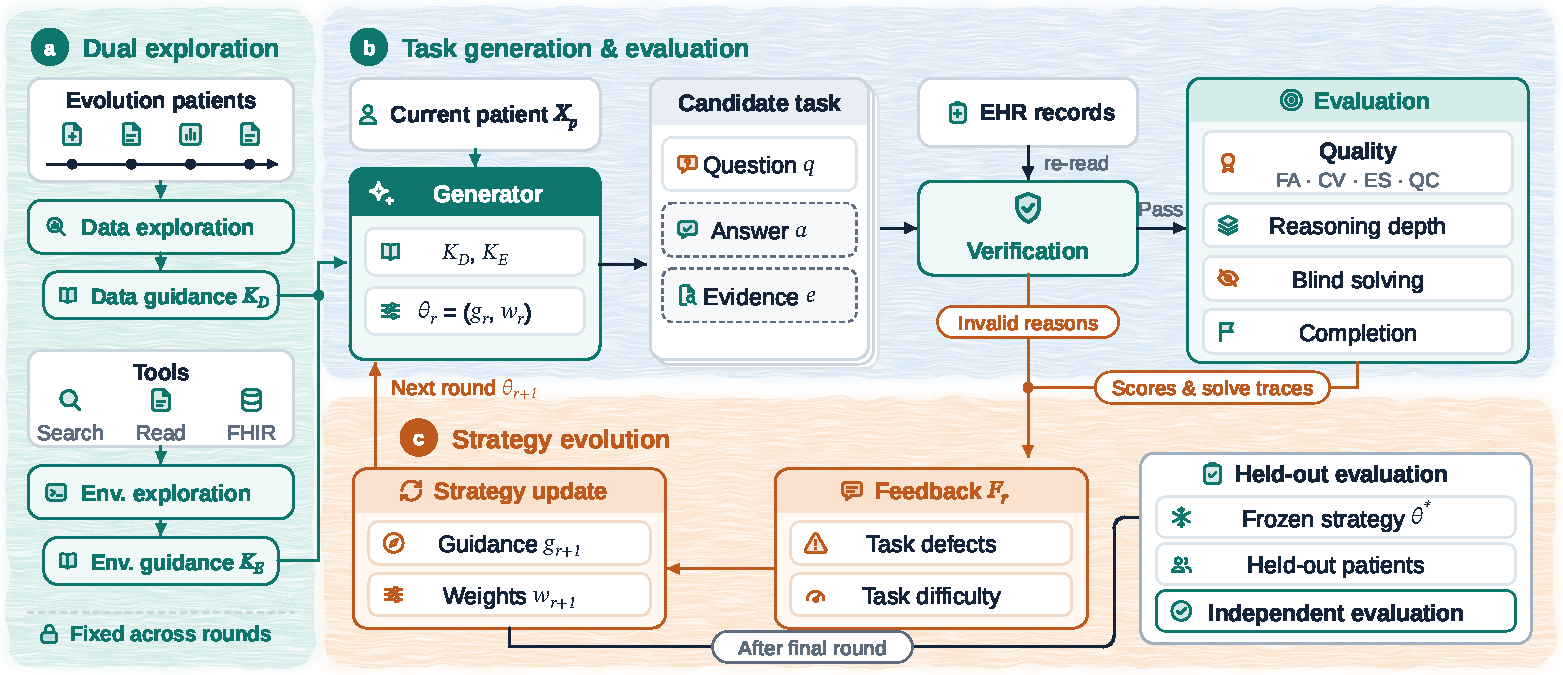
\includegraphics[width=\textwidth]{figures/medevolve-overview-v7.pdf}
\caption{MedEvolve 方法概览。（a）双探索分别从进化患者的纵向记录和只读工具交互中归纳数据指导 $K_D$ 与环境指导 $K_E$，在后续轮次中固定复用。（b）生成器以当前患者轨迹 $X_p$、两类探索指导与当前策略 $\theta_r=(g_r,w_r)$ 为条件生成候选任务，任务包含问题 $q$、参考答案 $a$ 与来源证据 $e$；核验重新读取原始记录，通过核验的任务进入质量（事实准确性 FA、临床合理性 CV、证据充分性 ES、题目清晰度 QC）、推理深度、独立解题与完成评价，参考答案与证据声明不提供给解题 Agent。（c）核验缺陷、评价得分与解题轨迹共同形成反馈 $F_r$，策略更新据此修订生成指导 $g_{r+1}$ 与方向权重 $w_{r+1}$；完成预定轮次后冻结策略 $\theta^*$，在独立患者集合上评测。}
\label{fig:overview}
\end{figure*}

\subsection{数据探索与环境探索}

单个患者的轨迹只说明该病例包含哪些记录，难以判断这些记录在整个数据源中属于何种模式，也无法在每次生成时重复读取大量患者。因此，我们在生成之前先进行数据探索，把跨患者的观察整理为可复用的指导。

\textbf{数据探索}针对纵向患者轨迹。探索 Agent 读取多位患者的记录，分析数据的组织方式、时间变化、临床事件之间的关联和证据分布，归纳出不同类型任务所需的信息模式，形成数据指导 $K_D$。$K_D$ 只描述可复用的模式，不包含特定患者的临床事实。

\textbf{环境探索}针对环境接口。探索 Agent 实际调用只读查询工具，记录访问方式、返回结构和交互约束，形成环境指导 $K_E$，用于判断一个问题所需的证据能否通过工具获取。

两类探索在初始化阶段完成，之后的所有轮次中保持不变。

\subsection{任务生成与评价}

对于患者 $X_p$，生成器以 $K_D$、$K_E$ 和当前策略 $\theta_r$ 为条件，按指定的任务类型和难度方向生成 $(q,a,e)$，其中关键事实附带对原始记录的引用。

候选任务随后依次经过核验、评分和独立解题。核验重新读取原始记录，检查证据声明对参考答案的支持；通过核验的任务再接受任务质量和推理深度的评价，并由固定的 Agent 在环境中独立作答。解题 Agent 无法获得参考答案和证据声明。

\subsection{反馈驱动的策略更新}

每轮结束后，系统汇总该轮任务的核验缺陷、质量与推理评分以及解题轨迹，归因得到反馈 $F_r$。归因需要区分任务本身的缺陷（如事实错误、证据不足、题意歧义）、任务带来的真实推理难度，以及模型、工具或环境故障，以避免将执行异常当作任务难度。策略按下式更新：
\begin{equation}
\theta_{r+1}=\mathcal{U}(\theta_r,F_r),
\end{equation}
其中 $\mathcal{U}$ 由 LLM 实现。更新作用于两个部分：一是把具有普遍性的构造经验写入 $g_{r+1}$，调整临床信息的选择、证据的组织和任务设计；二是根据各方向的质量与难度表现调整 $w_{r+1}$，改变后续任务的方向分布。

不同轮次使用不同的患者批次生成任务。完成预定轮次后冻结策略，并在独立的患者集上评测。

\section{实验}

\subsection{实验设置}

\textbf{环境与患者。}实验覆盖 PhysicianBench 与 MedAgentBench。PhysicianBench 有 108 位具有临床记录的患者；MedAgentBench 的 695 位患者中仅 100 位具有临床记录，实验使用这 100 位。按种子 42 划分后，PhysicianBench 的进化患者为 27 位、独立评测患者为 81 位，MedAgentBench 分别为 25 位和 75 位，两组患者互不重叠。各方法共享评测患者，每位患者最多生成两道只读任务，因此请求题数分别为 162 与 150。完整划分及信息访问规则见附录~\ref{app:env}。

\textbf{对比方法与模型。}比较六种生成方法：MedEvolve、TaskCraft、Workflow、SingleShot、SelfRefine（Madaan et al., 2023）和 EnvExplore，各方法的流程见附录~\ref{app:methods}。生成模型为 GPT-5.4-nano。MedEvolve 采用两轮更新后的完整策略，包括生成指导、题目方向描述及权重；两轮在 PhysicianBench 上分别使用 13 与 14 位进化患者，在 MedAgentBench 上分别使用 12 与 13 位。各方法的调用流程与计算投入不同，相同题数上限不代表相同计算成本。

\textbf{评价与指标。}生成的任务先对照原始记录核验，再进行难度评价。难度由 GPT-4o-mini 与 GPT-5.4-nano 两个裁判独立评分，取中位数并向下取整，得到 1–4 级的聚合层级。评分依据任务所需的最小充分推理路径；多条证据、长时间跨度、长答案或信息缺失本身不自动构成高阶推理。通过核验且聚合层级不低于 3 的任务称为高阶题。实验一使用三项指标：
\begin{itemize}
\item \textbf{高阶题数}：通过核验且层级不低于 3 的任务数。
\item \textbf{高阶产出率}：高阶题数除以固定的请求题数，生成失败和无效任务造成的损失计入其中。
\item \textbf{有效题平均层级}：全部通过核验且具有难度评分的任务的层级均值，并非仅对高阶题取平均，作为辅助指标。
\end{itemize}
指标分母及评分细则见附录~\ref{app:metrics}。

\subsection{实验一：有效高阶题生成}

该实验检验在相同患者和每患者题数上限下，各方法能否产出更多通过核验的高阶题。表~\ref{tab:exp1}~报告 GPT-5.4-nano 作为生成模型时的结果。

\begin{table*}[!t]
\centering
\small
\caption{高阶题生成比较（生成模型：GPT-5.4-nano）。产出率以请求题数为分母（PhysicianBench 162，MedAgentBench 150）；平均层级为全部通过核验题目的 1–4 级均值。}
\label{tab:exp1}
\setlength{\tabcolsep}{3pt}
\renewcommand{\arraystretch}{1.1}
\begin{tabularx}{\textwidth}{lYYYYYY}
\toprule
 & \multicolumn{3}{c}{PhysicianBench} & \multicolumn{3}{c}{MedAgentBench} \\
\cmidrule(lr){2-4}\cmidrule(lr){5-7}
方法 & 高阶题数 & 高阶产出率 & 平均层级 & 高阶题数 & 高阶产出率 & 平均层级 \\
\midrule
\textbf{MedEvolve} & \textbf{23} & \textbf{14.2\%} & 2.27 & \textbf{77} & \textbf{51.3\%} & 2.73 \\
TaskCraft & 0 & 0.0\% & 1.01 & 0 & 0.0\% & 1.00 \\
Workflow & 3 & 1.9\% & 2.30 & 2 & 1.3\% & 2.67 \\
SingleShot & 3 & 1.9\% & 1.20 & 11 & 7.3\% & 1.44 \\
SelfRefine & 4 & 2.5\% & 2.20 & 2 & 1.3\% & 2.00 \\
EnvExplore & 21 & 13.0\% & 2.25 & 64 & 42.7\% & 2.56 \\
\bottomrule
\end{tabularx}
\end{table*}

MedEvolve 在两个环境中的高阶题数和产出率均最高，分别产出 23 题（14.2\%）与 77 题（51.3\%）。相比 SingleShot 的 3 题与 11 题，以及 SelfRefine 的 4 题与 2 题，MedEvolve 的高阶题数高出数倍至数十倍；TaskCraft 没有产出高阶题，平均层级接近 1，其任务以事实查询为主。最接近的方法是 EnvExplore，为 21 题与 64 题，即在同样使用环境探索的基础上，MedEvolve 的完整策略在 PhysicianBench 上多产出 2 题，在 MedAgentBench 上多产出 13 题；本实验未做区间估计，PhysicianBench 上的差距较小，不据此判断显著差异。

高阶产出率以固定的请求题数为分母，生成失败和未通过核验的任务造成的损失都已计入，因此上述优势是在扣除这些损失之后得到的。Workflow 与 SelfRefine 的实际生成量很小，也是其产出率低的原因之一。各方法的生成与核验数量见附录~\ref{app:counts}（表~\ref{tab:counts}）；MedEvolve 的核验通过率低于 TaskCraft 等方法，其优势体现在高阶题的数量，而非核验通过率。有效题平均层级的方法间差距小于高阶题数的差距，且 Workflow 在 PhysicianBench 上的均值（2.30）略高于 MedEvolve（2.27），但仅基于 10 道通过核验的题目，因此该指标只作辅助参考。

\subsection{实验二：合成任务补充官方任务训练}

该实验检验在官方任务训练之外加入 MedEvolve 合成任务，能否改善 Agent 在官方测试任务上的表现。环境为 PhysicianBench，比较 ACE、Reflexion（Shinn et al., 2023）和 OpenClaw 三个框架。执行模型为 Qwen3.8-27B，关闭思考，模型参数保持固定，各框架通过自身的记忆、反思或策略机制从训练任务中积累经验。

比较两种训练设置。“官方 20”使用 20 道官方任务；“官方＋合成 40”在同一批 20 道官方任务之外，加入 20 道通过核验的 MedEvolve 合成任务，其中 GPT-4o-mini 与 GPT-5.4-nano 生成的各 10 道。两组均在共同的 50 道官方测试任务上评价，模型调用预算为 100，种子为 42。参考答案只用于评分，不提供给执行与学习过程；训练结束后冻结经验再进行测试。框架机制与评测细节见附录~\ref{app:exp2}。

\begin{table}[!t]
\centering
\small
\caption{官方任务训练加入合成任务前后的题目通过率。通过率以全部 50 道计划测试题为分母，表示严格的整题成功。}
\label{tab:exp2}
\setlength{\tabcolsep}{3pt}
\begin{tabularx}{\columnwidth}{lYYY}
\toprule
框架 & 官方 20 & 官方＋合成 40 & 差值 \\
\midrule
ACE & 4.0\%（2/50） & 10.0\%（5/50） & $+6.0$ pp \\
Reflexion & 12.0\%（6/50） & 14.0\%（7/50） & $+2.0$ pp \\
OpenClaw & 24.0\%（12/50） & 20.0\%（10/50） & $-4.0$ pp \\
\bottomrule
\end{tabularx}
\end{table}

评分覆盖方面，ACE 的官方 20 组覆盖 48 题、混合组覆盖 50 题，Reflexion 与 OpenClaw 的两组均覆盖 50 题。

加入合成任务后，ACE 与 Reflexion 的题目通过率分别提高 6.0 与 2.0 个百分点，OpenClaw 则下降 4.0 个百分点，三个框架的变化方向并不一致。这些结果只说明在所观察的设置内各框架的变化，不能证明合成任务带来稳定、普遍的下游收益，也不能证明收益由高阶题本身造成。患者隔离的多种子补充实验仍在进行，尚无最终结果。

\raggedbottom

\section{结论}

MedEvolve 通过数据与环境双探索选择由当前病例支持的问题，再利用核验和解题反馈跨患者更新生成指导与方向权重，整个过程不更新模型参数。在 PhysicianBench 与 MedAgentBench 上，相同患者和每患者题数上限下，MedEvolve 产出的通过核验的高阶题最多，但其核验通过率低于部分基线，说明有效性与推理要求需要联合评价。将合成任务补充到官方任务训练后，不同框架的题目通过率变化不一致，目前不足以支持稳定的下游收益结论。

\section*{局限性（Limitations）}

病例记录的完整性、时间信息和模型输入预算限制了可发现的提问模式，轨迹裁剪也可能遗漏关键依据。同一环境内的患者独立划分只能检验该环境中的迁移，跨机构或跨数据来源的泛化仍需另外评价。当前生成采用回顾性信息访问，不启用时间视角隔离，因此不代表临床当时可获得的信息范围。

难度评价由两个模型的评分聚合而来，不能消除二者共有的偏差；高阶题数的方法间差异也未附区间估计。各方法的调用流程与计算投入不同，相同题数上限不代表相同计算成本。本文没有开展组件消融，因此无法分别归因数据探索、环境探索和反馈更新各自的贡献；多轮反馈更新的效果也未在本文评价。

下游实验仅在 PhysicianBench 的三个框架上进行，结果为单种子，50 道测试题上相差一到数题属于较大的不确定性；患者隔离的多种子补充实验仍在进行。该结果不能证明稳定的下游收益，也不能证明收益来自高阶题本身。不同框架的原生学习机制不同，比较限定在同一框架内。

\section*{参考文献}

Jiang, Yixing, et al. 2025. \href{https://arxiv.org/abs/2501.14654}{MedAgentBench: A Realistic Virtual EHR Environment to Benchmark Medical LLM Agents}. arXiv:2501.14654.

Liu, Ruoqi, et al. 2026. \href{https://arxiv.org/abs/2605.02240}{PhysicianBench: Evaluating LLM Agents in Real-World EHR Environments}. arXiv:2605.02240.

Shi, Dingfeng, et al. 2025. \href{https://arxiv.org/abs/2506.10055}{TaskCraft: Automated Generation of Agentic Tasks}. arXiv:2506.10055.

Mai, Shinji, et al. 2025. \href{https://arxiv.org/abs/2512.01311}{CuES: A Curiosity-driven and Environment-grounded Synthesis Framework for Agentic RL}. arXiv:2512.01311.

Shinn, Noah, et al. 2023. \href{https://arxiv.org/abs/2303.11366}{Reflexion: Language Agents with Verbal Reinforcement Learning}. arXiv:2303.11366.

Zhai, Yunpeng, et al. 2025. \href{https://arxiv.org/abs/2511.10395}{AgentEvolver: Towards Efficient Self-Evolving Agent System}. arXiv:2511.10395.

Madaan, Aman, et al. 2023. \href{https://arxiv.org/abs/2303.17651}{Self-Refine: Iterative Refinement with Self-Feedback}. arXiv:2303.17651.

Kassis, Timothy, Vinayak Agarwal, Yuhuan He, Darshil Patel, and Aubrey M. Brueckner. 2026. \href{https://arxiv.org/abs/2609.00065}{Scientific Agent Skills: A Library of Procedural Knowledge for Research Agents}. https://doi.org/10.48550/arXiv.2609.00065.

\appendix

\section{探索与生成接口}

\subsection{数据探索}

探索工具提供开放患者名单、预算内轨迹及可选压缩摘要。输入材料保留患者标识、原始来源和覆盖标记，输出为不绑定患者的自然语言指导。指导归纳数据组织、时间变化、事件关系、证据引用与可支持的问题，不保留个体临床值或来源编号。

压缩摘要用于定位模式，原始记录用于支持具体事实。记录缺失与材料裁剪分别解释。指导中的时间窗口、记录数量或临床关系属于模型归纳的提问约束，不构成对所有患者统一适用的硬编码医学规则。

\subsection{环境探索}

环境探索在独立实例中访问开放患者的原生只读工具。指导记录已验证参数、返回结构、分页与裁剪行为、典型检索方式，并区分调用失败和未验证能力。环境内的具体患者观察不进入通用指导。

\subsection{指导修订实例}

\begin{figure}[!t]
\centering
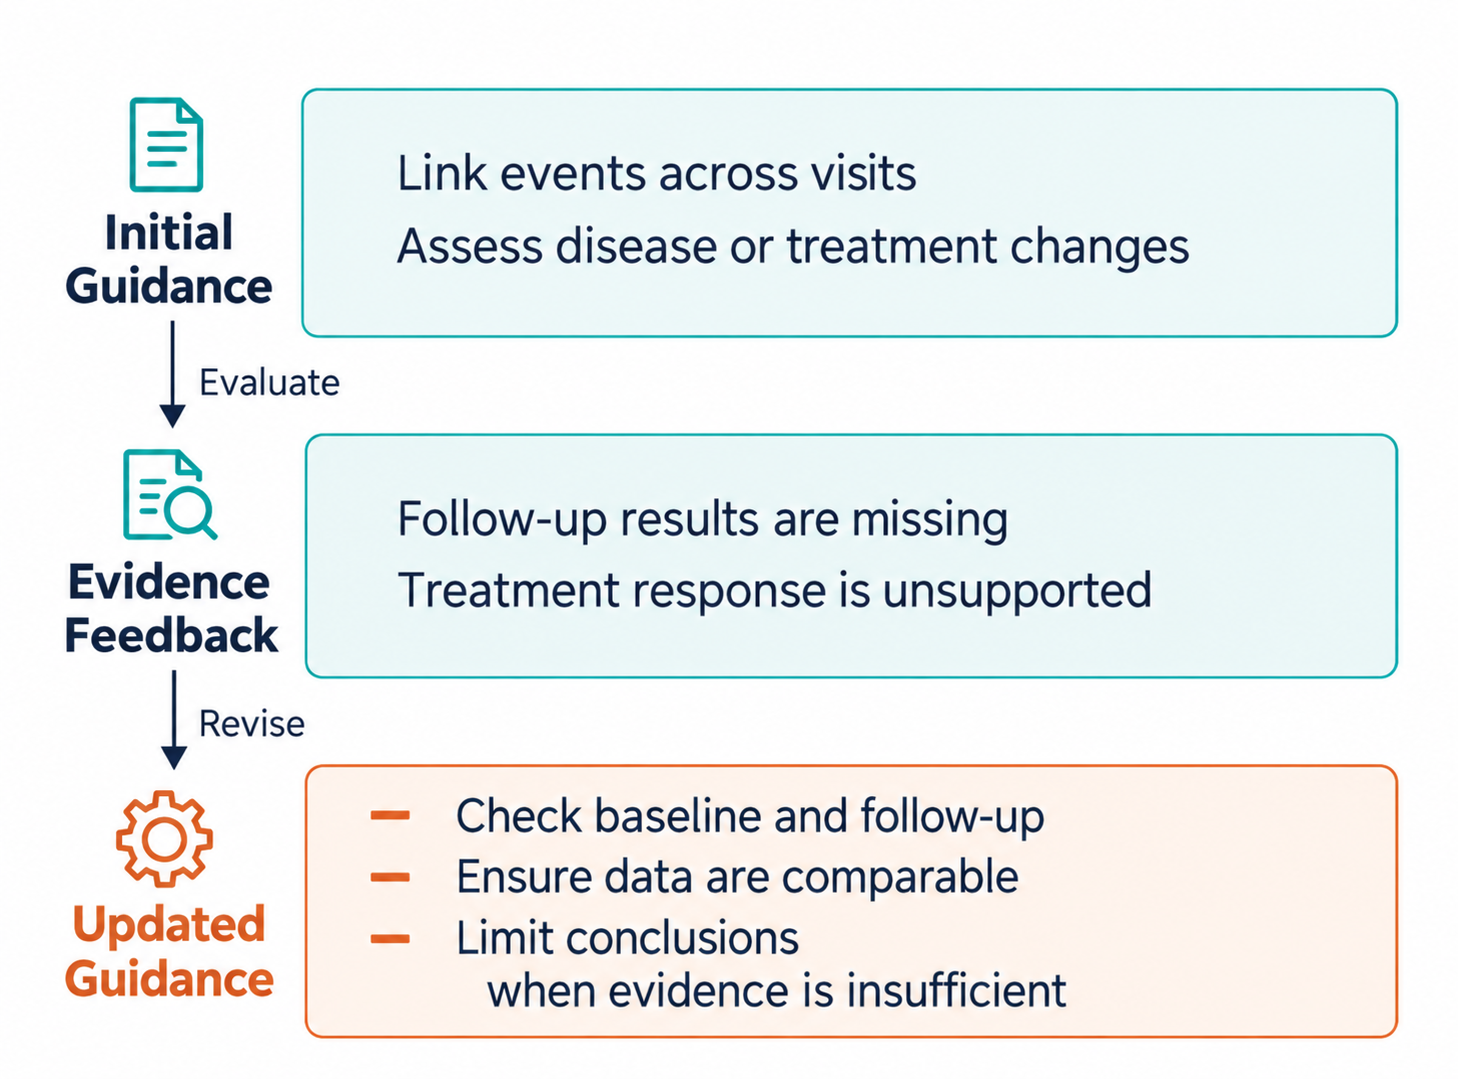
\includegraphics[width=\columnwidth]{figures/medevolve-strategy-example-en.png}
\caption{一次策略自进化中的指导修订。核验反馈指出随访证据不足，更新后的指导增加基线、随访与数据可比性检查，并限定证据不足时的结论。图中文字根据一次进化记录概括。}
\end{figure}

\subsection{任务生成与策略}

任务包含患者标识、临床题型、问题、候选参考答案、来源标识与逐来源事实声明，以及执行要求；当前公共生成接口要求时间视角字段为空，执行要求为只读。生成调用输入预算内轨迹、两类探索指导、当前生成指导和两个采样方向，输出最多两题。

生成策略由自然语言指导和方向列表组成；方向包含五类临床题型之一、难度描述与非负权重。方向按权重采样，允许同一题型对应不同临床模式；至少一个权重为正。数据与环境指导在策略更新期间固定，更新只修订生成指导和方向列表。进化与评测阶段均按当前方向权重抽样，评测阶段使用冻结后的完整策略，即生成指导与方向权重。

\section{环境、患者与信息访问}
\label{app:env}

\begin{table}[!t]
\centering
\small
\caption{生成侧患者划分。}
\setlength{\tabcolsep}{3pt}
\begin{tabularx}{\columnwidth}{lYYYY}
\toprule
环境 & 患者总数 & 进化集 & 评测集 & 两轮进化患者数 \\
\midrule
PhysicianBench & 108 & 27 & 81 & 13 / 14 \\
MedAgentBench & 100 & 25 & 75 & 12 / 13 \\
\bottomrule
\end{tabularx}
\end{table}

PhysicianBench 的生成患者池为 108 人，MedAgentBench 为官方范围内的 100 人。按种子 42 和既有探索暴露约束冻结进化与评测名单。进化患者分为互不重叠的两轮：PhysicianBench 为 13 与 14 人，MedAgentBench 为 12 与 13 人；评测患者分别为 81 与 75 人。

原始轨迹按记录时间组织，模型输入按预算选取；证据核验读取原始来源，不以输入摘要替代来源。初始探索和任务生成只开放查询工具。解题工具依环境与任务执行要求提供，经验训练的合成任务进一步限定为只读。当前公共生成接口未启用时间视角属性，问题中的时间限定不等同于服务端隐藏后续记录。

实验二的训练任务为 20 道官方任务加 20 道通过核验的合成任务，测试任务为共同的 50 道官方任务，该划分与生成侧患者划分相互独立。冻结清单记录选中题目、患者、训练与测试划分、文件摘要及生成来源。

\section{生成方法与预算}
\label{app:methods}

TaskCraft 将患者记录与只读 FHIR 工具映射到原方法的结论抽取、原子任务生成、核验与扩展流程。深度和宽度分支均从原子任务出发，彼此没有先后依赖；两条分支共享生成总预算。原子、深度和宽度候选的实际产量及接纳情况分别记录，以区分扩展机制和最终筛选的影响。医疗适配与原论文完整实验复现分别解释。

Workflow 固定执行定位、生成和内部检查，检查只筛选候选。SingleShot 根据轨迹单次生成最多两题。SelfRefine 在同一患者批次内执行初稿、自反馈和修订，最多三次自评、两次修订，全部通过时提前结束。EnvExplore 先获取环境指导，再用固定初始策略生成任务。各方法共享输出结构和公共评价，内部调用与筛选记录分别保存。

主方法初始探索完成后执行两轮生成侧策略进化，每轮按患者归纳反馈并汇总更新。批次输出的结构或配额校验失败保留为生成失败。反馈和更新调用失败不视为进化成功。输入裁剪、实际调用与预算耗尽分别记录。

模型路由、上下文上限、输出限制和工具预算以冻结运行配置为准。同一比较中报告各方法预算与实际用量；相同出题数量不表述为严格相同 token 预算。探索和更新计入主方法总成本，公共评价成本单列，历史复用调用按原始记录去重计数。

\section{评分与指标}
\label{app:metrics}

\subsection{推理层级}

推理层级依据问题要求及证据结构标注：第 1 级直接读取事实，第 2 级结合记录与临床知识完成单步判断，第 3 级跨记录比较或整合信息，第 4 级综合证据权衡风险收益并提出方案。评分依据完成任务所需的最小充分推理路径；证据数量、时间跨度、答案长度或信息缺失本身不自动提高层级。临床题型与推理层级分别记录，不把治疗规划题自动判为最高层级。

对任务 $i$，两个裁判模型给出的原始层级为 $l_i^{(1)}$ 与 $l_i^{(2)}$，聚合层级为
\[
l_i=\left\lfloor\operatorname{median}\left(l_i^{(1)},l_i^{(2)}\right)\right\rfloor.
\]
聚合层级不低于 3 且通过核验的任务记为高阶题。正式协议要求两份有效输出，不以单个成功裁判替代缺失评价，原始层级与理由保留用于分歧分析。

\subsection{指标与分母}

\begin{table*}[!t]
\centering
\small
\caption{指标定义与分母。}
\setlength{\tabcolsep}{3pt}
\renewcommand{\arraystretch}{1.15}
\begin{tabularx}{\textwidth}{lYY}
\toprule
指标 & 分子 & 分母 \\
\midrule
高阶题数 & 通过核验且聚合层级不低于 3 的题数 & — \\
高阶产出率 & 高阶题数 & 固定请求题数 \\
有效题平均层级 & 通过核验且具有难度评分的题目的层级之和 & 通过核验且具有难度评分的题数 \\
核验通过率 & 核验通过题数 & 实际生成题数 \\
题目通过率（实验二） & 严格整题成功的测试题数 & 计划测试题数（50） \\
\bottomrule
\end{tabularx}
\end{table*}

生成失败和无效任务保留在产出统计中，不从分母中剔除。实验二的评分故障保留为覆盖不足，不转换为失败或成功。

\section{经验学习与官方评测}
\label{app:exp2}

\begin{table*}[!t]
\centering
\small
\caption{三种框架的经验载体与更新机制。}
\setlength{\tabcolsep}{3pt}
\renewcommand{\arraystretch}{1.15}
\begin{tabularx}{\textwidth}{lYYY}
\toprule
框架 & 持久化经验 & 训练更新 & 测试状态 \\
\midrule
OpenClaw & 技能与独立状态目录 & 原生 Skill Workshop，记录是否触发 & 读取冻结技能，关闭学习与后台维护 \\
ACE & 策略手册 & Reflector 和 Curator 更新 & 只运行 Generator \\
Reflexion & 反思与可迁移经验 & 失败反思及限定次数重试 & 只运行 Actor，读取经验 \\
\bottomrule
\end{tabularx}
\end{table*}

两种训练设置各自独立保存配置和经验，从统一初始状态开始。Reflexion 的跨任务经验提炼为医疗适配：保存适用条件、操作步骤和错误教训，不保存患者标识、个体临床值或逐题答案；新题按冻结规则读取最多三条相关经验。测试不根据评分进行反思或重试。

执行模型为 Qwen3.8-27B，关闭思考，模型调用预算为 100，种子为 42。官方 20 题是两种训练设置共用的训练任务；混合设置另加入 20 道通过核验的 MedEvolve 合成任务，由 GPT-4o-mini 与 GPT-5.4-nano 各生成 10 道。

PhysicianBench 使用官方任务和检查点评分，提供实际文件交付、执行轨迹和本题 FHIR 实例；官方资产缺失或评分故障保留为不可用结果，不以公共模型裁判替代原生分数。参考答案只用于评分，不提供给执行与学习过程。

测试评分与解题隔离，评分完成前保留实际使用的医疗实例。每题使用冻结经验副本，不将参考答案、评分结果或完整会话回写到最终经验。测试前后核对冻结经验摘要，报告计划任务数与评分覆盖。

\section{生成与核验数量}
\label{app:counts}

\begin{table*}[!t]
\centering
\small
\caption{各方法的生成与核验数量（生成模型：GPT-5.4-nano，冻结旧批次）。分数为实际生成题数／核验通过题数；通过率为核验通过题数除以实际生成题数。}
\label{tab:counts}
\setlength{\tabcolsep}{3pt}
\renewcommand{\arraystretch}{1.1}
\begin{tabularx}{\textwidth}{lYYYY}
\toprule
方法 & PhysicianBench 生成／通过 & 通过率 & MedAgentBench 生成／通过 & 通过率 \\
\midrule
MedEvolve & 157／70 & 44.6\% & 146／104 & 71.2\% \\
TaskCraft & 128／125 & 97.7\% & 111／108 & 97.3\% \\
Workflow & 32／10 & 31.3\% & 11／3 & 27.3\% \\
SingleShot & 162／122 & 75.3\% & 150／127 & 84.7\% \\
SelfRefine & 12／10 & 83.3\% & 7／6 & 85.7\% \\
EnvExplore & 149／107$^\dagger$ & 71.8\%$^\dagger$ & 141／108 & 76.6\% \\
\bottomrule
\end{tabularx}
\end{table*}

$^\dagger$ PhysicianBench 上 EnvExplore 的数量来自冻结的旧批次，与表~\ref{tab:exp1}~中 21 道高阶题所在的最新运行不是同一批，不能作为这 21 题的分母。

\section{写作辅助工具}

中文稿的结构组织、方法描述核对与证据状态检查使用 Scientific Agent Skills 的 scientific-writing 技能（Kassis et al., 2026）辅助。文献与科学结论的最终核验由作者负责。

\end{document}
